\documentclass{article}
\usepackage[utf8]{inputenc}
\usepackage[spanish]{babel}
\usepackage{graphicx}	%Si se quiere compilar con las imagenes
% \usepackage[draft]{graphicx}	%Si NO se quiere compilar con las imagenes porque tarda mucho
\usepackage{graphics, float, fancyhdr, titling, caption, subcaption}
\usepackage{listings}
\usepackage[a4paper, total={6in, 9.5in}]{geometry}
\usepackage{fancyhdr}
\usepackage{hyperref}   %para que funcione addcontentsline debe ser la ultima que se cargue
\usepackage{amsmath}
%\setcounter{secnumdepth}{-2}       %Poner solo esto si no se quieren numero delante de las secciones y niveles inferiores.

\renewcommand{\footrulewidth}{0.4pt}
\title{

\includegraphics[width=1.75in]{imagenes/UGR-Logo.png} \\
\vspace*{1in}
\textbf{Memoria de la práctica 3} \\
Animación por Ordenador \\
\vspace*{0.5in}}
\author{Andrés Merlo Trujillo \\
andresmerlo@correo.ugr.es \\
77147239H \\ 
\vspace*{0.5in} \\
E.T.S. de Ingenierías Informática y de Telecomunicación \\
\textbf{Universidad de Granada}} \date{\today}

\hypersetup{
    colorlinks=true,
    linkcolor=black,
    citecolor=black
}

\renewcommand\maketitlehooka{\null\mbox{}\vfill}
\renewcommand\maketitlehookd{\vfill\null}

\begin{document}
\begin{titlingpage}
\maketitle
\end{titlingpage}

\tableofcontents

\newpage

\pagestyle{fancy}   %a partir de comienza el header (se salta el indice y portada)
\fancyhead[L]{Andrés Merlo Trujillo}
\fancyhead[R]{Animación por Ordenador}
%\section{Ejercicio 1}
%\begin{figure}[H]
%    \centering
%    \includegraphics[width=\textwidth]{imagenes/passwdfile.png}
%    \vspace{10pt}
%    \footnotesize{Fuente: https://...}
%\end{figure}

% \begin{figure}[H]
%     \centering 
% 	\begin{subfigure}[t]{0.48\textwidth}
% 	    \centering
% 	    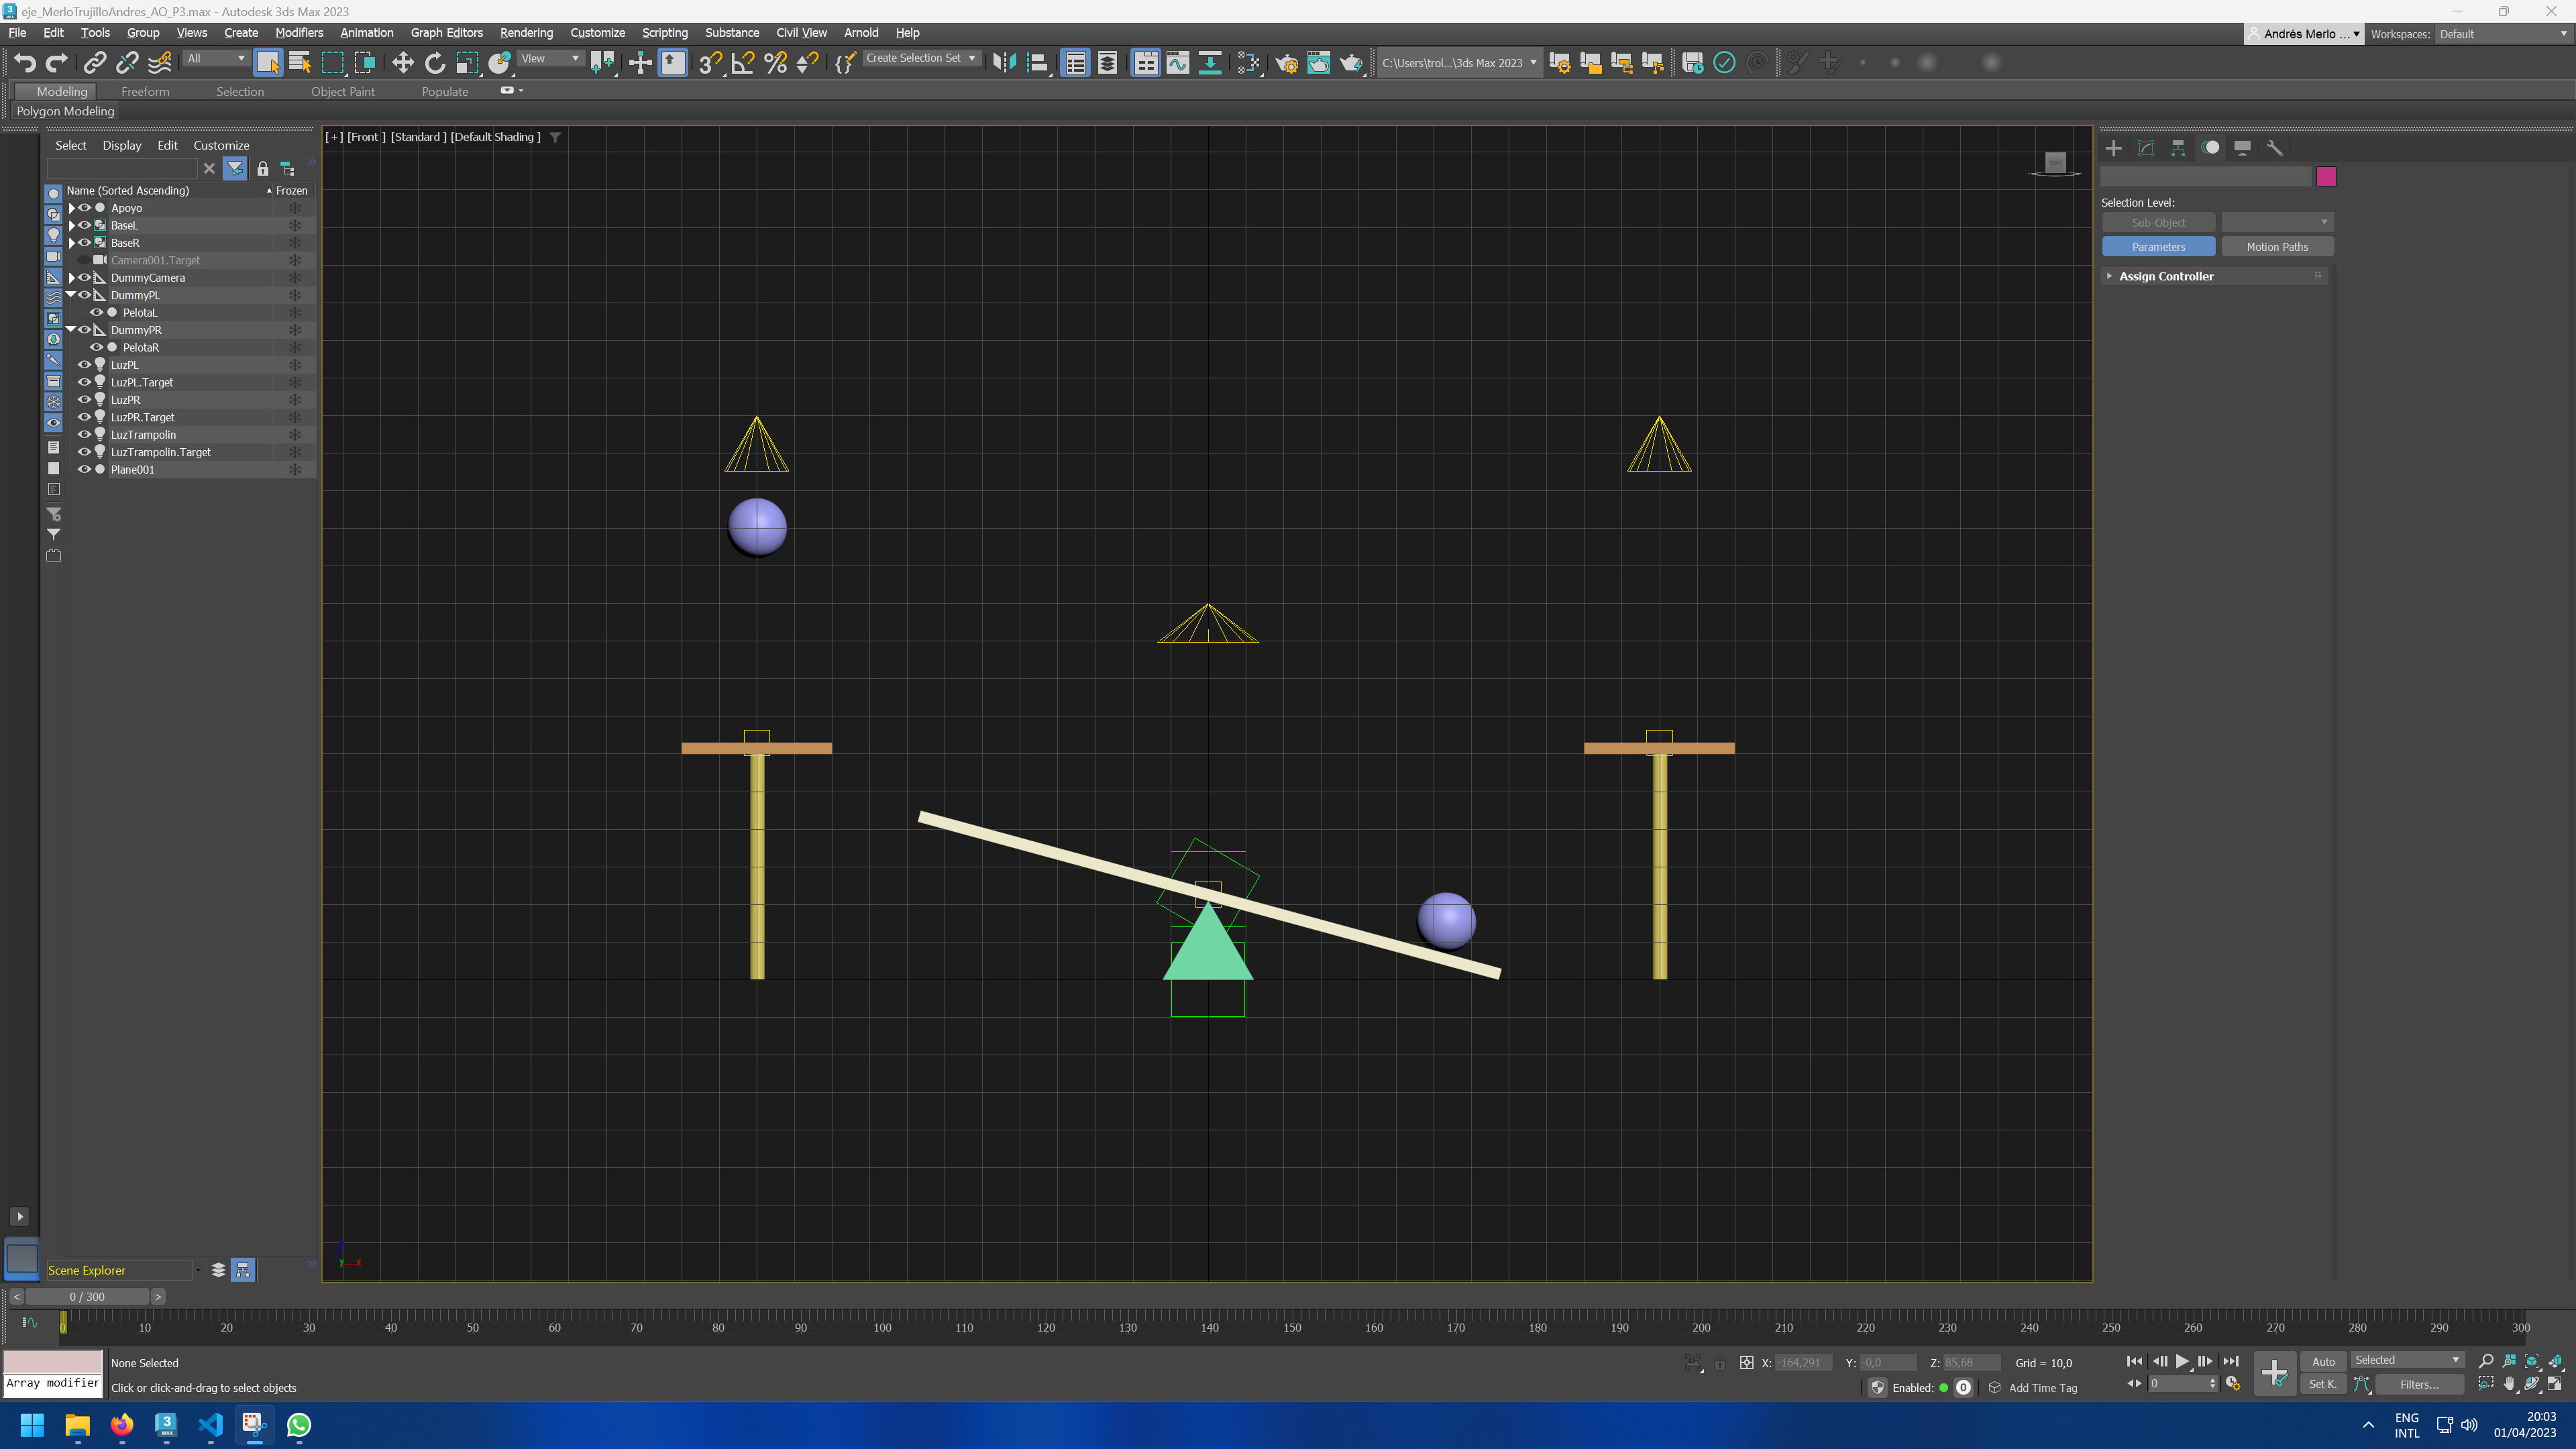
\includegraphics[width=\textwidth]{imagenes/Ejercicio 1/keyframes/0.png}
%         \caption{Pelotas en el instante 0.}
%     \end{subfigure}
%     \hfill
%     %\par\bigskip %si se desea dejar un margen entre la imagen de arriba y de abajo
% 	\begin{subfigure}[t]{0.48\textwidth}
% 	    \centering
% 	    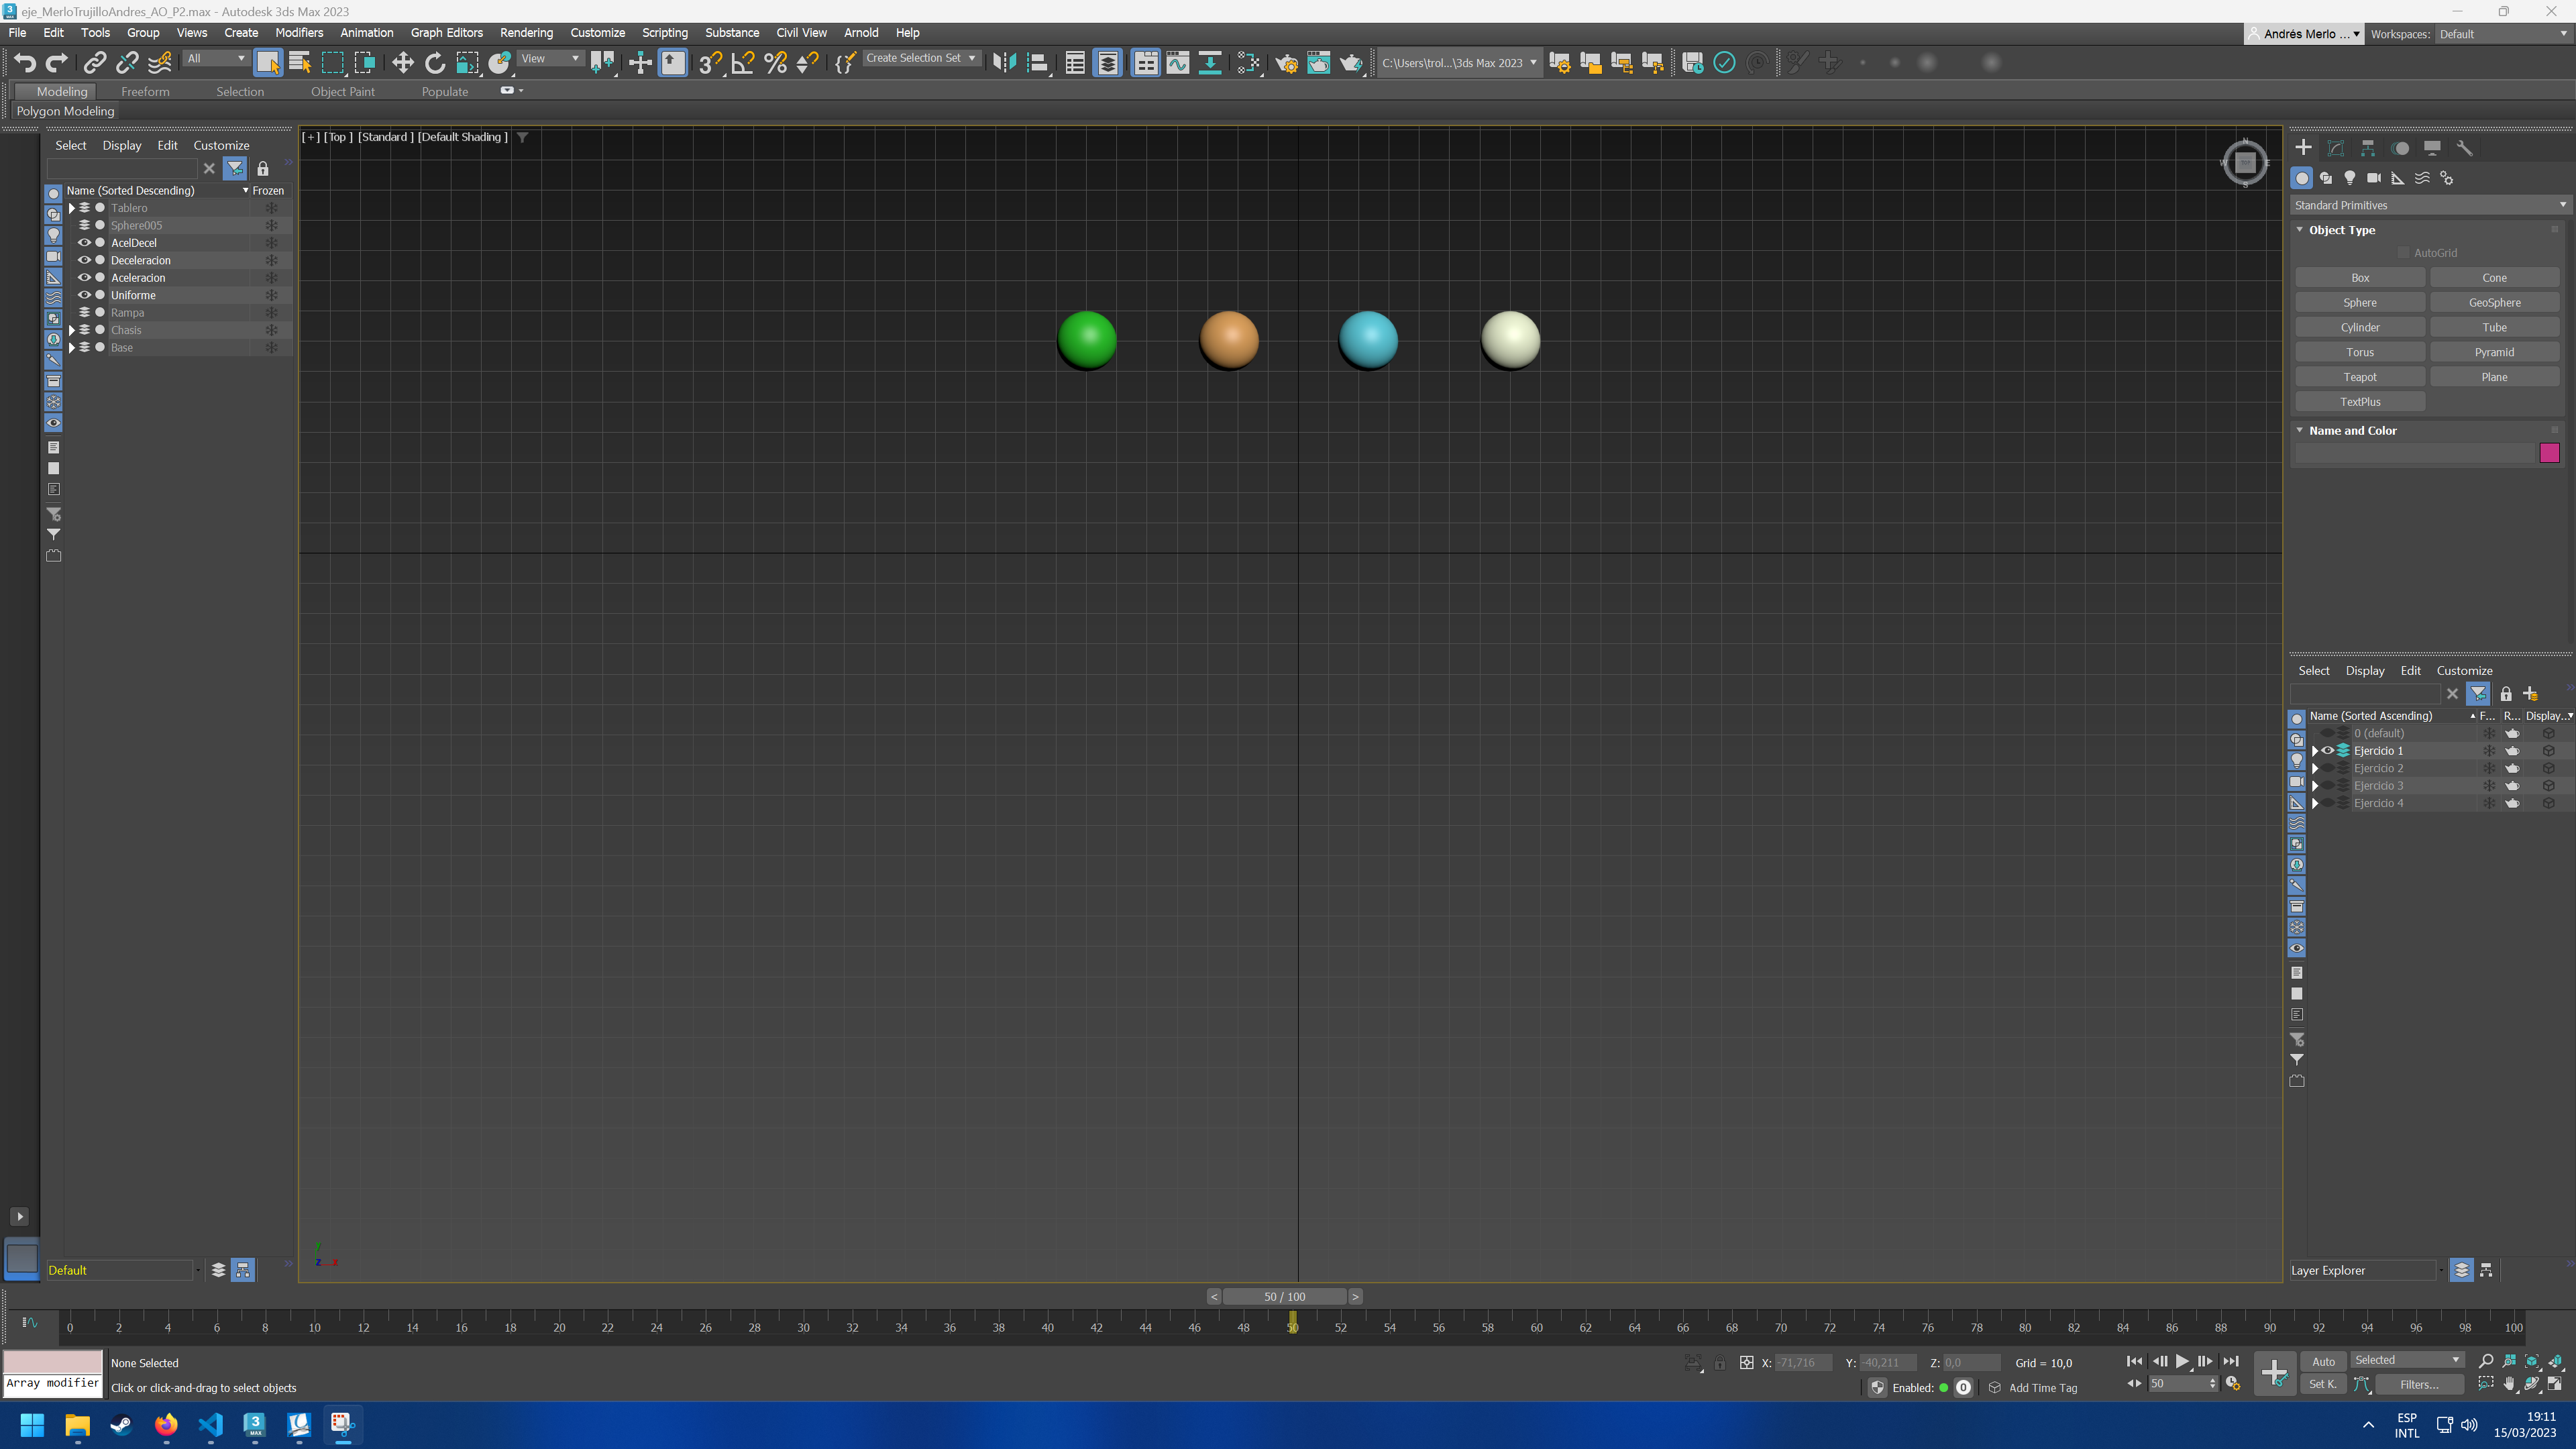
\includegraphics[width=\textwidth]{imagenes/Ejercicio 1/keyframes/50.png}
%         \caption{Pelotas en el instante 50.}
%     \end{subfigure}    
% \end{figure}


\section{Introducción}
% rescribir
En esta práctica se pide animar un conjunto de pelotas, que rebotan y caen a un balancín, haciendo que la otra rebote y caiga en una plataforma. También se debe animar un conjunto de luces que iluminará la parte de la escena que está en movimiento actualmente y una cámara, que rotará alrededor de la escena.

Todo lo mencionado anteriormente se debe \textit{loopear} de forma invertida, de manera que cuando acabe la animación vuelva a realizarse, pero al revés, comenzando por el final y acabando por el principio.

En esta memoria voy a dividir cada una de las partes que he realizado en secciones, las cuales se encontrarán a continuación.

\section{Número de fotogramas}

% rescribir
En la práctica se pedía que la animación durase 5 segundos, y otros 5 segundos haciendo la animación inversa. 

En mi caso, he usado 30 fotogramas por segundo, los que pone por defecto 3ds Max. Por tanto los cálculos para obtener lo números de fotogramas necesarios son los siguientes:


$30 \text{ fps} \times 2 \times 5 \text{ segundos} = 300 \text{ fotogramas} $

\end{document}
